\section{Methodology}\label{sec-metodologia}

Systematic literature reviews represent methodological approaches that seek to identify, evaluate, and interpret trends in a given field of study \cite{Garcia-Penalvo2022}. As it is an emerging transdisciplinary conceptual proposal, we consider it the most appropriate to outline the debate on AL in this investigation. Designed to reduce bias and provide evidence to support academic debates, systematic literature reviews involve a series of steps, such as introduction, planning, carrying out, and reporting the review \cite{White2005}. In this article, we structure each stage based on four questions \Cref{tab-01}. Defining research questions is the most important step in a systematic literature review, as it establishes the basis that guides decisions throughout the research process, thus seeking to effectively contribute to the production of knowledge about gaps in a given literature (García-Peñalvo, 2022).
In our study, the questions are constructed from four axes of investigation into the idea of AL: a) its conceptual proposals, b) the techniques and pedagogical strategies emerging in these debates, c) functions and spaces for applying this knowledge. and, finally, d) the challenges and difficulties depicted in the literature. Based on these axes, we identified four guiding questions for the review, which is presented in \Cref{tab-01}.

\begin{table}[!htpb]
\centering
\begin{threeparttable}
\caption{Guiding questions for the systematic literature review process on AL}
\label{tab-01}
\begin{tabular}{p{0.97\textwidth}}
\toprule
Q1: What are the conceptual models that make up AL and how do these proposals differ from other forms of literacy, such as digital or media literacy? \\
Q2: What are the pedagogical approaches related to AL and how do they work in promoting knowledge and awareness about the action of algorithms? \\
Q3: What are the main activities or areas of knowledge in which algorithmic literacy is applied? \\
Q4: What are the main obstacles faced in the development of algorithmic literacy, considering different factors such as education, access to technology, and digital culture? \\
\bottomrule
\end{tabular}
\source{Created by the authors.}
\end{threeparttable}
\end{table}
    
The process of selecting the publications analyzed in this article was inspired by the so-called PRISMA statement \cite{Moher2009}, which is configured as an analysis flow with four phases for systematic reviews. The present investigation adopted the first three stages of the PRISMA statement (identification, screening and eligibility), as we consider that they account for the process of qualifying the selection of publications to be analyzed and of reducing bias.

\Cref{image-01} shows the selection flow of publications analyzed in this systematic review on LA. In Phase 1, Identification, the initial capture of publications, we use two important databases, Scopus and Web of Science. Their choice was based on scope and academic reputation. Both platforms are known for indexing a wide spectrum of scientific journals, conferences and other relevant sources, ensuring a comprehensive and diverse search for publications on the topic. Furthermore, Scopus and Web of Science have advanced filtering and search capabilities, allowing the use of specific descriptors in multiple languages, such as Portuguese, English, and Spanish, which enabled a multilingual approach in identifying articles and research related to LA. The search was conducted using terms in the three languages. In Portuguese and Spanish, we used the descriptors ‘Literacy AND Algorithmic’. For the English language, we used the descriptors ‘algorithmic OR algorithm AND literacy OR literacies’. In the search system of both platforms, terms were searched in the title, abstract, and keywords of the publications. At the end of the search process, we identified a total of 42 publications in Scopus and 25 in Web of Science.

\begin{figure}[h!]
\centering
\begin{minipage}{0.85\textwidth}
\caption{Selection flow of publications to be analyzed.}
\label{image-01}
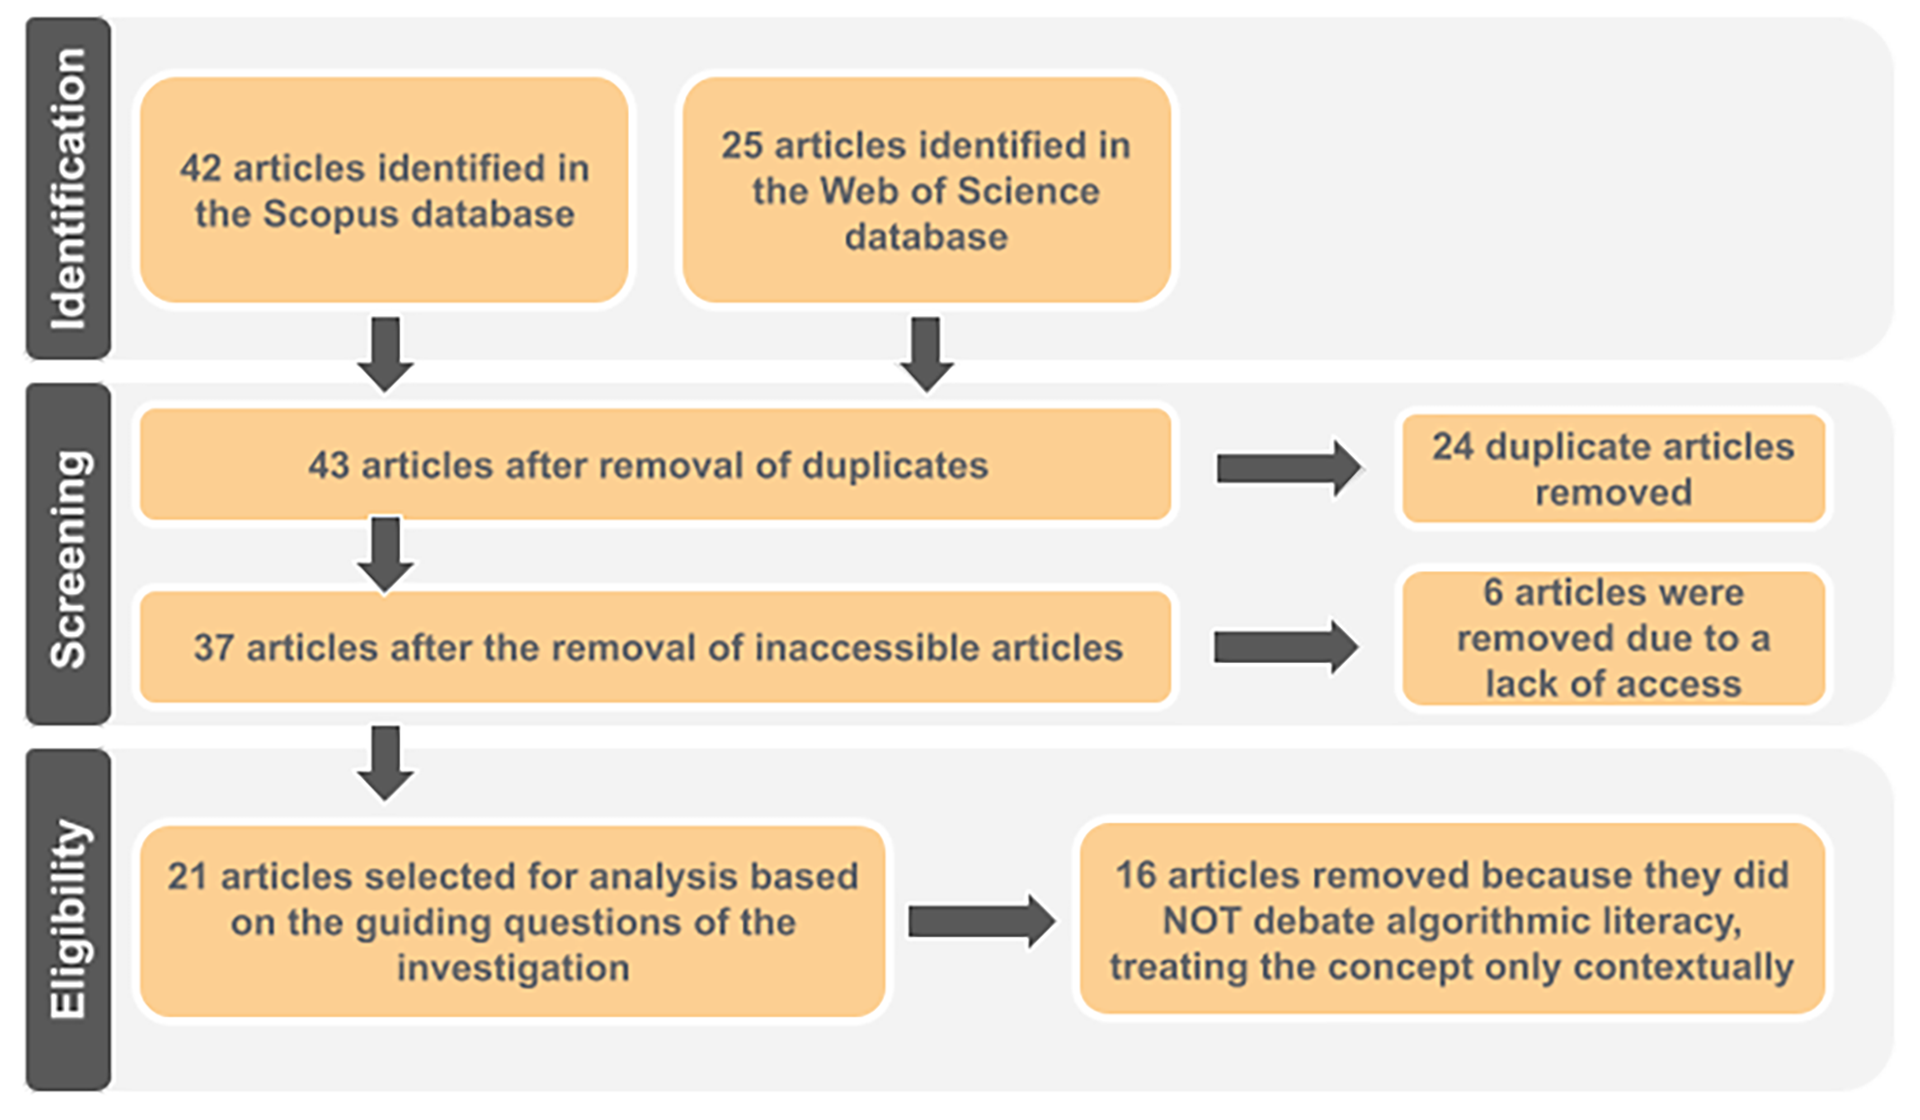
\includegraphics[width=\linewidth]{image1_en.png}
\source{Created by the authors.}
\end{minipage}
\end{figure}

In the screening phase, 24 duplicate publications were identified, that is, studies that appeared on both search platforms. Furthermore, during the screening, six publications were considered inaccessible by the researchers. These works could not be obtained for different reasons: subscription restrictions, payment on certain platforms, or unavailability of the full text by the authors or magazines. The decision to remove these inaccessible publications was made based on the need to ensure the reliability and completeness of the review, as the inability to access the full content could negatively affect the analysis and interpretation of results.

After identifying and removing duplications and inaccessible publications, 37 articles remained for the eligibility phase. At this stage, inclusion and exclusion criteria become essential. Such definitions are established to ensure that the analytical focus of the guiding questions is reflected in the selection of publications, providing greater clarity and efficiency to the analysis process. As shown in \cref{tab-02}, the inclusion criteria include studies that address the concept of AL, as well as present proposals and reflections on practices intended to generate AL, in addition to articles written in Portuguese, English, or Spanish published up to the cut-off date of this review (December 2022). The exclusion criteria seek to eliminate studies whose full text was unavailable at the time of data collection, works unrelated to AL, and studies in which AL is addressed only as a contextual element for the analysis of a more specific theme.

   
\begin{table}[!htpb]
\centering
\begin{threeparttable}
\caption{Critérios de seleção para fase de elegibilidade}
\label{tab-02}
\begin{tabular}{p{0.475\textwidth} p{0.475\textwidth}}
\toprule
Inclusion criteria & Exclusion criteria \\
\midrule
Studies that address the concept of AL. & Studies that did not have the full text available to researchers at the time of data capture. \\
Studies that present proposals and reflections on practices intended to generate AL. & Studies that are not related to AL. \\
Articles written in Portuguese, English, or Spanish. & Studies in which AL is used only as a contextual element to analyze a more specific theme. \\
Publications available until the cut-off date of this review (December 2022). &  \\
\bottomrule
\end{tabular}
\source{Created by the authors.}
\end{threeparttable}
\end{table}   


In the Eligibility stage, the analysis process consisted of a thorough reading of the texts of the publications, together with the production of summaries about each study and its main findings. From these summaries and the original texts, the eligibility analysis was conducted. The most preponderant exclusion criterion was the elimination of publications that do not deepen the discussion on the concept of algorithmic literacy or do not present training or pedagogical proposals related to the topic (in total, 16). In these publications, algorithmic literacy appears as a side discussion, generally acted as an imperative for contemporary education, without substantially exploring its meaning or possible applications. We can cite the article by \textcite[p. 759]{Cotter2020}, which analyzes how the socioeconomic context continues to shape the use of digital technologies and deepen disparities, which indicates that “greater algorithmic literacy can also imply familiarity with the functioning of algorithms, as well as the ability to evaluate their informative results”. Although they highlight the relevance of algorithmic literacy, there is no debate about what exactly comprises this concept. Similarly, \posscite{Kapsch2022} article, which explores how young adults make sense of and reflect on their agency as users in relation to algorithms, sees algorithmic literacy as a possible result of the study's methodological proposal, without actually outlining a systematic definition. Still in this group of works eliminated in the eligibility phase, there are a series of studies that place AL as a tool for learning mathematics and computing \cite{Astambayeva2021,How2022}, an approach that distances itself from the objectives and issues guiding our study.
